\subsection{Advanced Composition Explorer}

The Advanced Composition Explorer (ACE) is a satellite that is positioned between the Earth and the sun, close to the first Lagrangian point (L1) and about 1.5 million km from the Earth. This gives the satellite a good view at the solar wind. It carries different systems with it including SWEPAM and MAG
\begin{wrapfigure}{r}{0.5\textwidth} 
\vspace{-20pt}
  \begin{center}
    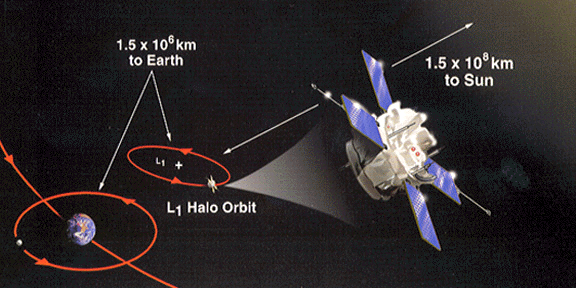
\includegraphics[width=0.4\textwidth]{Figures/ACE/ace_l1.png}
    \caption{Placement of ACE between the Earth and Sun.}
    \label{fig:ACE}
  \end{center}
  \vspace{-20pt}
  \vspace{1pt}
\end{wrapfigure}

The Magnetic Field experiment (MAG)
Looks at the fluctuations of the interplanetary magnetic field(IMF). 

The Solar Wind Electron Proton Alpha Monitor(SWEPAM) provides the bulk solar wind observations 